编写良好的DPC++内核没有工作项依赖关系,就可以在CPU上高效地并行,还可以对DPC++内核应用向量化,以利用SIMD硬件。实际上,CPU处理器可以使用SIMD指令优化内存负载、存储和操作,因为大多数数据元素通常位于连续内存中,并且通过数据并行内核采用相同的控制流。例如,有a[i] = a[i] + b[i]语句的内核中,通过在多个数据元素之间共享硬件逻辑,并将它们作为一个组执行,每个数据元素都以相同的指令流load、load、add和store操作,可以自然地映射到硬件的SIMD指令集。因此,一个指令可以同时处理多个数据元素。\par

由一条指令同时处理的数据元素的数量,有时称为指令或执行指令的处理器的向量长度(或SIMD宽度)。图16-11中,指令流以4路SIMD执行运行。\par

\hspace*{\fill} \par %插入空行
图16-11 SIMD的指令流
\begin{center}
	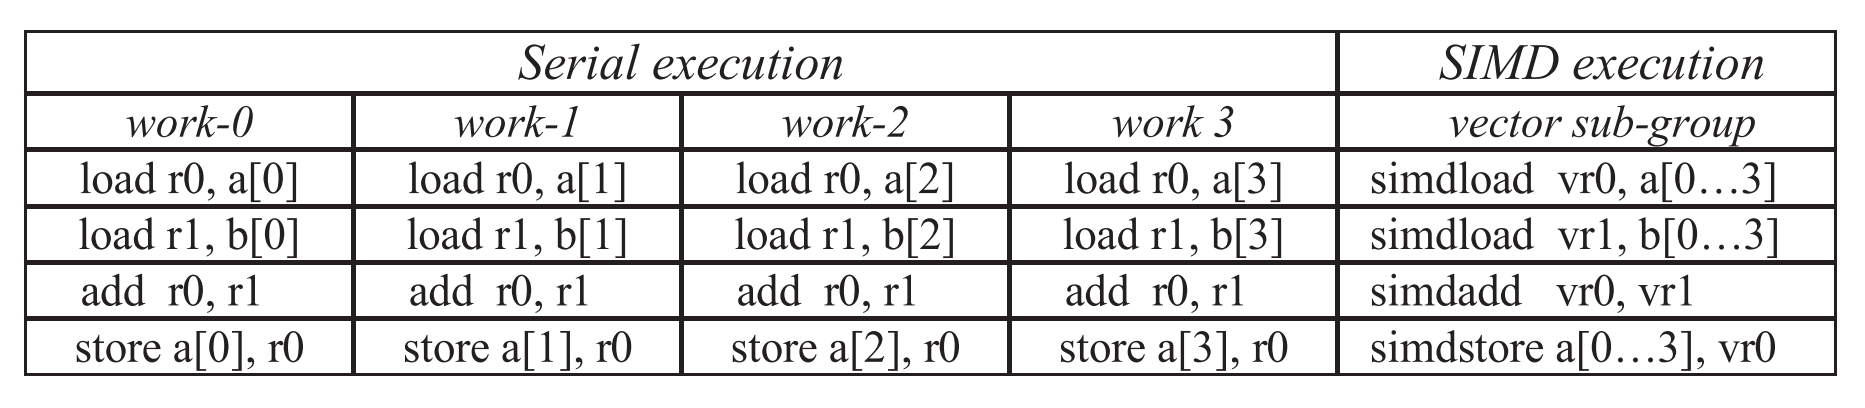
\includegraphics[width=1.0\textwidth]{content/chapter-16/images/10}
\end{center}

CPU处理器并不是唯一实现SIMD指令集的处理器。其他处理器(如GPU)实现SIMD指令以提高处理大型数据集的效率。与其他处理器类型相比,Intel Xeon CPU处理器的区别是有三个固定大小的SIMD寄存器宽度(128位XMM、256位YMM和512位ZMM),而不是一个可变长度的SIMD。当使用子工作组或向量类型编写具有SIMD并行性的DPC++代码时,需要注意硬件中的SIMD宽度和SIMD向量寄存器的数量。\par

\hspace*{\fill} \par %插入空行
\textbf{确保SIMD执行的合法性}

DPC++执行模型确保SIMD执行可以应用于任何内核,以及每个工作组中的一组工作项(即一个子工作组)可以使用SIMD指令并发执行。有些实现可以选择使用SIMD指令在内核中执行循环,只有保留所有原始数据依赖关系,或者保留由编译器基于语义解析的数据依赖关系才有可能。\par

使用工作组内的SIMD指令,可以将单个DPC++内核执行从单个工作项的处理转换为一组工作项。在ND-Range模型下,生成SIMD代码的编译器向量器选择了增长最快的(单位步幅)维度。实际上,要启用给定ND-Range的向量化,在同一子工作组中的任何两个工作项之间,不应该存在依赖关系,或者编译器需要在同一子工作组中保留工作项向前依赖关系。\par

当工作项的内核执行映射到CPU上的线程时,细粒度同步的代价很高,线程上下文切换的开销也很高。因此,为CPU编写DPC++内核时,消除工作组内工作项之间的依赖对性能优化很重要。另一种有效的方法是依赖子工作组中的工作项,如图16-12中“先读后写”的依赖。如果子工作组是在SIMD执行模型下执行的,那么编译器可以将内核中的子工作组栅栏忽略,在运行时不会产生同步成本。\par

\hspace*{\fill} \par %插入空行
图16-12 使用子工作组向量化具有前向依赖性的循环
\begin{lstlisting}[caption={}]
using namespace sycl::intel;

queue Q;
range<2> G = {n, w};
range<2> L = {1, w};

int *a = malloc_shared<int>(n*(n+1), Q);

for (int i = 0; i < n; i++)
	for (int j = 0; j < n+1; j++) a[i*n + j] = i + j;
	
Q.parallel_for(nd_range<2>{G, L}, [=](nd_item<2> it)
	[[cl::intel_reqd_sub_group_size(w)]] {
		
	// distribute uniform "i" over the sub-group with 8-way
	// redundant computation
	const int i = it.get_global_id(0);
	sub_group sg = it.get_sub_group();
	
	for (int j = sg.get_local_id()[0]; j < n; j += w) {
		// load a[i*n+j+1:8] before updating a[i*n+j:8] to preserve
		// loop-carried forward dependence
		auto va = a[i*n + j + 1];
		sg.barrier();
		a[i*n + j] = va + i + 2;
	}
	sg.barrier();
	
}).wait();
\end{lstlisting}

内核向量化(向量长度为8),其SIMD执行如图16-13所示。工作组的规模为(1,8),内核的循环迭代分布在这些子工作组工作项上,并以8路SIMD并行方式执行。\par

本例中,如果内核中的循环控制性能,那么允许跨子工作组的SIMD向量化将有显著的性能改进。\par

使用并行处理数据元素的SIMD指令,是让内核的性能超出CPU内核和超线程数量的方法。\par

\hspace*{\fill} \par %插入空行
图16-13 具有前向依赖关系的循环的SIMD向量化
\begin{center}
	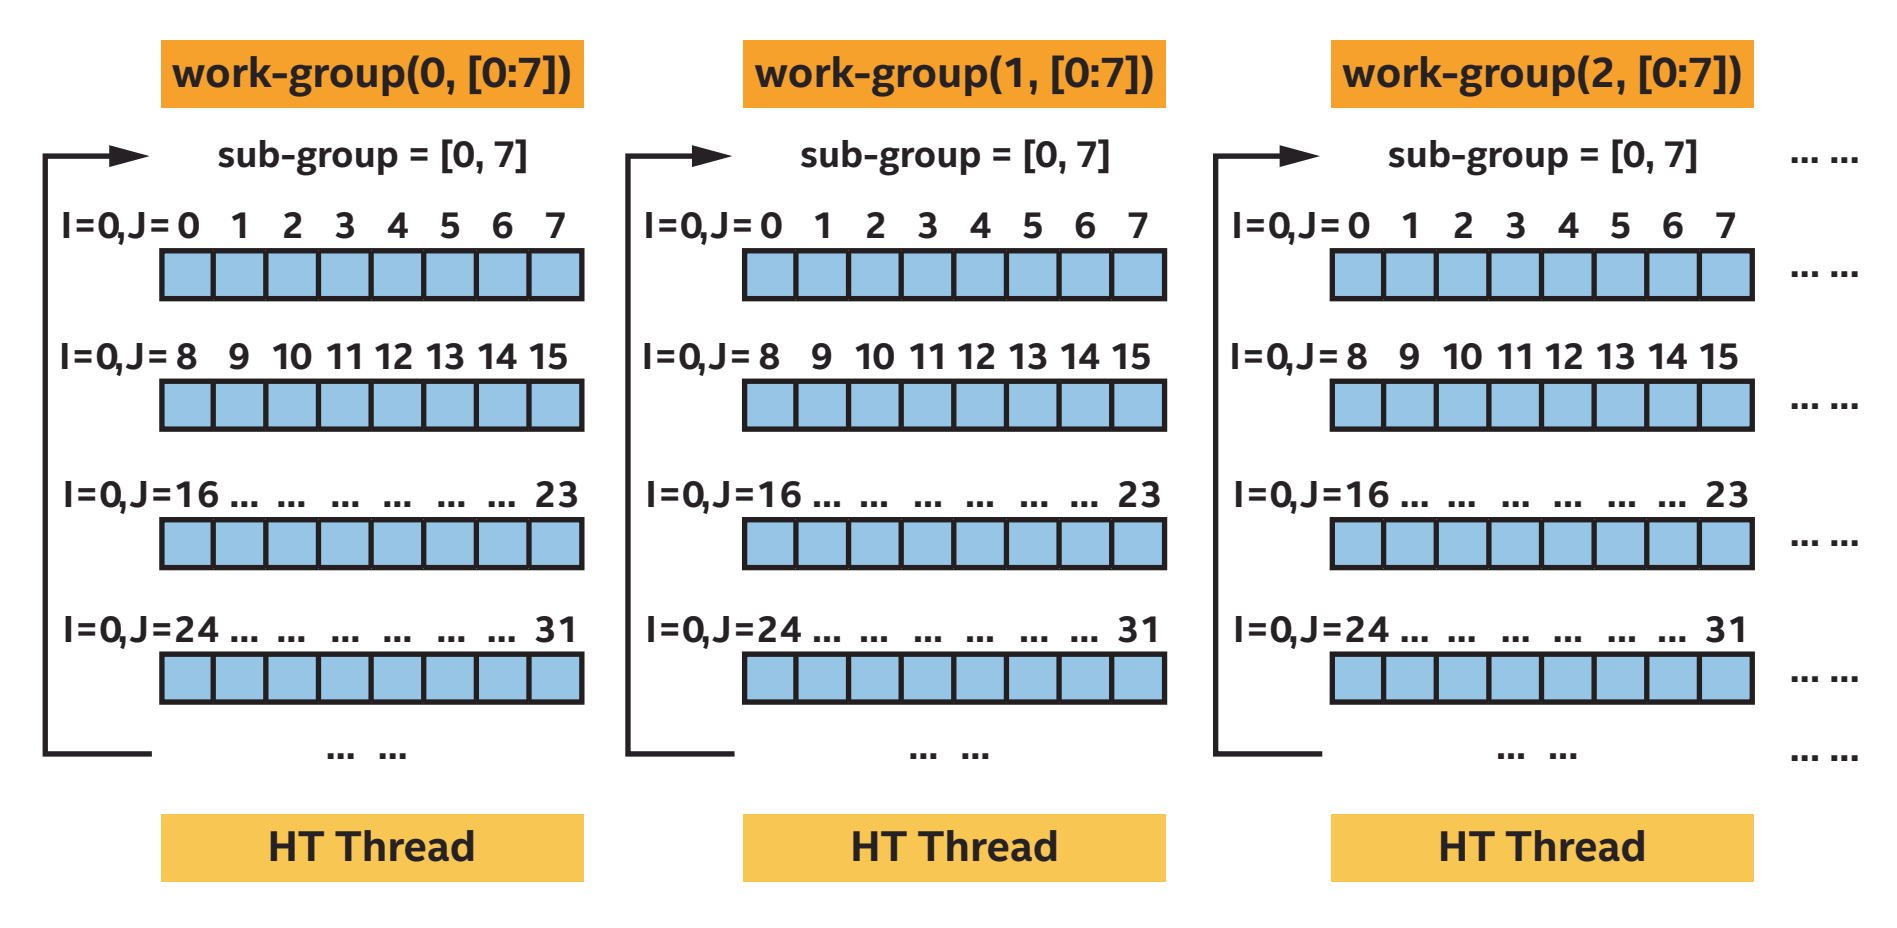
\includegraphics[width=1.0\textwidth]{content/chapter-16/images/7}
\end{center}

\hspace*{\fill} \par %插入空行
\textbf{SIMD掩码和成本}

实际应用中,我们可以期待条件语句,如if语句,条件表达式,如a = b > a?A: b,迭代次数可变的循环,switch语句等等。任何条件可能导致标量控制流不执行相同的代码路径,就像在GPU(第15章),可能会导致性能下降。SIMD掩码是一组值为1或0的位,由内核中的条件语句生成。考虑一个例子,A={1,2,3,4}, B={3,7,8,1},以及比较表达式A < B。比较返回一个掩码,包含四个值{1,1,1,0},可以存储在硬件掩码寄存器中,以指示以后哪些通道的SIMD指令应该执行比较所保护(使能)的代码。\par

内核包含条件代码,与基于与每个数据元素相关联的掩码位(SIMD指令中的通道)执行向量化的掩码指令。每个数据元素的掩码位与掩码寄存器中的位置相对应。\par

使用掩码可能会导致性能低于相应的非掩码代码。这可能是由于以下原因:\par

\begin{itemize}
	\item 负载上附加了掩码操作
	\item 对目标的依赖
\end{itemize}

掩码是有成本的,所以只在必要时使用。当内核是具有执行范围内工作项显式分组的ND-Range内核时,在选择ND-Range工作组大小,通过最小化掩码成本来最大限度地提高SIMD效率时应格外小心。当工作组的大小不能被处理器的SIMD宽度均匀整除时,工作组的一部分可能会被内核忽略。\par

\hspace*{\fill} \par %插入空行
图16-14 内核中使用的三种掩码
\begin{center}
	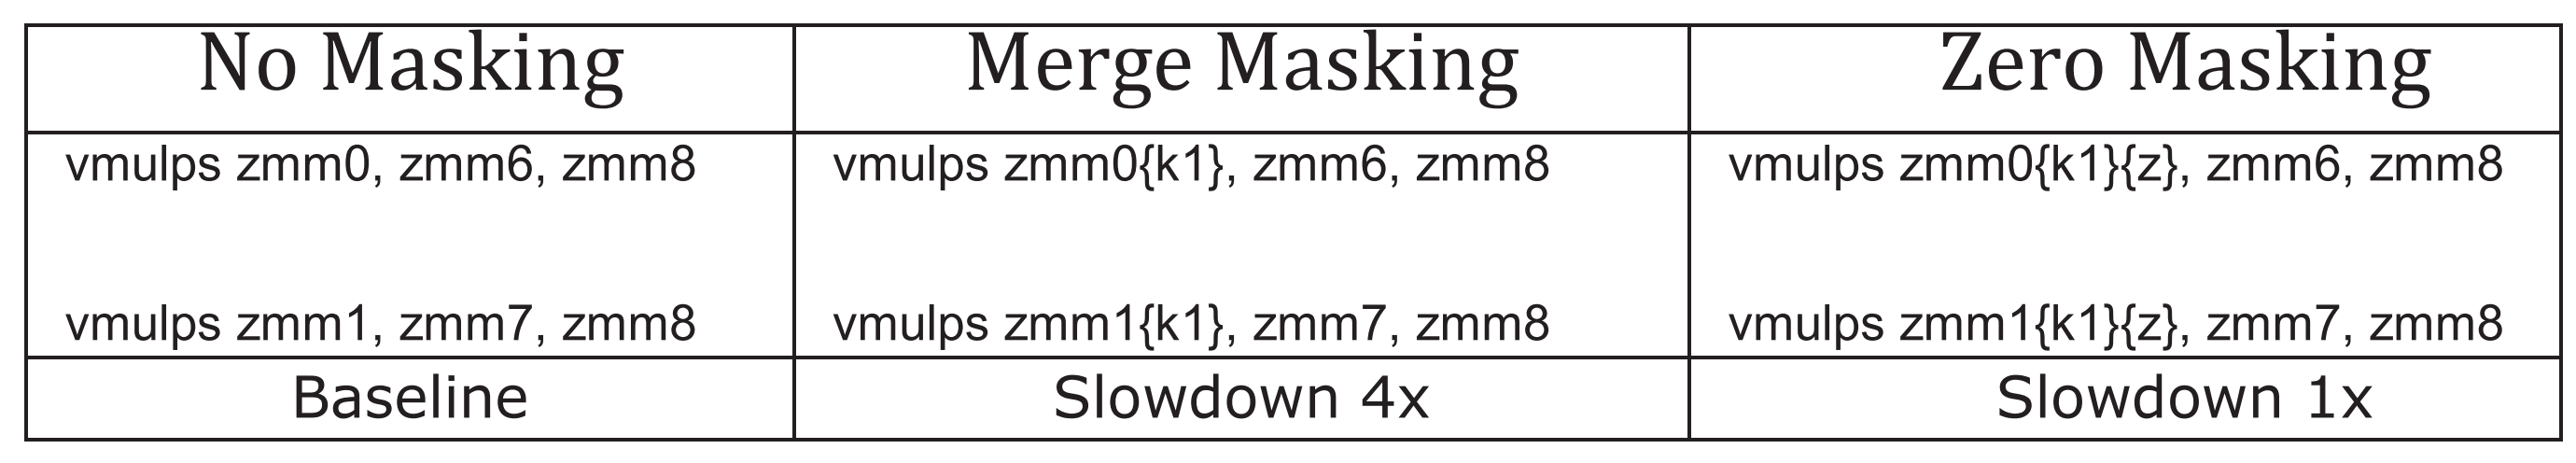
\includegraphics[width=1.0\textwidth]{content/chapter-16/images/11}
\end{center}

图16-14显示了如何使用合并掩码创建一个依赖于目标寄存器:\par

\begin{itemize}
	\item 如果没有掩码,处理器每个周期执行两个乘法(vmulps)。
	\item 合并掩码时,处理器每四个周期执行两次乘法,因为乘法指令(vmulps)保存在目的寄存器中,如图16-17所示。
	\item 零屏蔽不依赖于目标寄存器,因此在每个周期执行两个乘法(vmulps)。
\end{itemize}

访问缓存对齐的数据比访问非对齐的数据具有更好的性能。地址在编译时未知,或者是未对齐的,这种情况下,可以剥离对内存的访问,使用掩码访问处理前几个元素,直到第一个对齐的地址,然后通过并行内核中的多版本控制技术处理未掩码的访问,随后是忽略剩余数。这种方法增加了代码大小,但从整体上改善了数据处理性能。\par

\hspace*{\fill} \par %插入空行
\textbf{避免使用结构数组来提高SIMD效率}

AOS(结构数组)结构会影响SIMD的效率,也会为内存访问带来额外的带宽和延迟。硬件聚集-分散机制的存在并不能消除这种转换的需求——聚集-分散访问通常需要比连续负载更高的带宽和延迟。给定一个AOS数据布局struct \{float x; float y; float z; float w;\} a[4],考虑一个内核在它上面操作,如图16-15所示。\par

\hspace*{\fill} \par %插入空行
图16-15 SIMD在内核中聚集
\begin{lstlisting}[caption={}]
cgh.parallel_for<class aos<T>>(numOfItems,[=](id<1> wi) {
	x[wi] = a[wi].x; // lead to gather x0, x1, x2, x3
	y[wi] = a[wi].y; // lead to gather y0, y1, y2, y3
	z[wi] = a[wi].z; // lead to gather z0, z1, z2, z3 
	w[wi] = a[wi].w; // lead to gather w0, w1, w2, w3
});
\end{lstlisting}

当编译器沿着一组工作项向量化内核时,由于是非单位步长的内存访问,会导致SIMD收集指令的生成。例如,a[0].x, a[1].x, a[2].x和a[3].x的跨距是4,,不是更有效的步幅1。\par

\begin{center}
	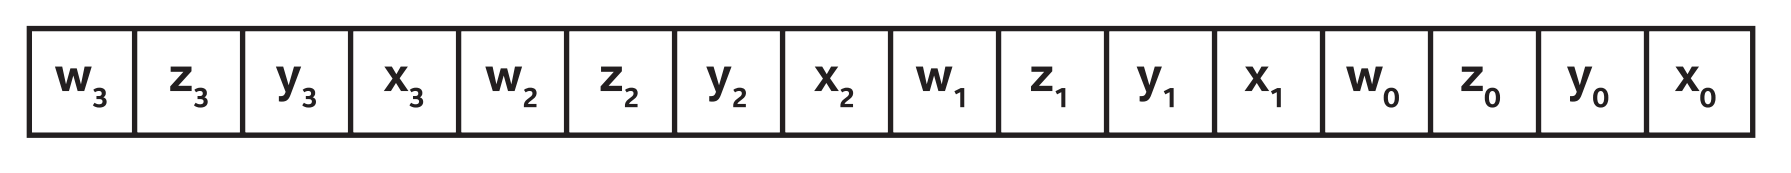
\includegraphics[width=1.0\textwidth]{content/chapter-16/images/8}
\end{center}

内核中,通常可以通过消除对内存收集-分散操作的使用来实现更高效的SIMD。一些代码可以从数据布局中获益,这些将以结构数组(Array-of-Struct, AOS)表示形式编写的数据结构转换为阵列结构(Structure of Arrays, SOA),在执行SIMD向量化时,为每个结构字段使用单独的数组以保持内存访问的连续性。例如,考虑这样一个SOA数据布局:struct {float x[4]; float y[4]; float z[4]; float w[4];} a; 如下所示:\par

\begin{center}
	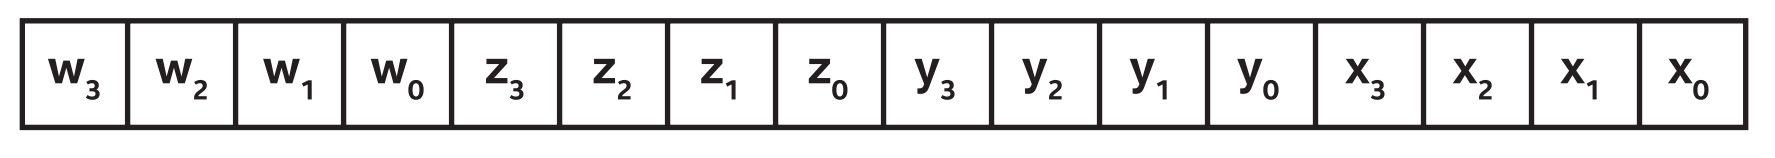
\includegraphics[width=1.0\textwidth]{content/chapter-16/images/9}
\end{center}

内核可以使用如图16-16所示的单位步长(连续)向量加载和存储数据,即使是向量化!

\hspace*{\fill} \par %插入空行
图16-16 SIMD操作单位跨距的内核
\begin{lstlisting}[caption={}]
cgh.parallel_for<class aos<T>>(numOfItems,[=](id<1> wi) {
	x[wi] = a.x[wi]; // lead to unit-stride vector load x[0:4]
	y[wi] = a.y[wi]; // lead to unit-stride vector load y[0:4]
	z[wi] = a.z[wi]; // lead to unit-stride vector load z[0:4]
	w[wi] = a.w[wi]; // lead to unit-stride vector load w[0:4]
});
\end{lstlisting}

SOA数据布局有助于在跨数组元素访问结构的一个字段时防止聚集,并帮助编译器对与工作项相关的连续数组元素上的内核进行向量化。考虑到使用这些数据结构的地方,希望在程序级别完成这些AOS-to-SOA或AOSOA的数据布局转换。仅在循环级别上执行此操作将涉及循环前后格式之间的转换。我们还可以依赖编译器对AOS数据布局进行向量加载和混洗优化,但要付出一定的代价。如果SOA(或AOS)数据布局的成员具有向量类型,那么编译器向量化将执行第11章中描述的基于底层硬件的水平扩展或垂直扩展,以生成最佳代码。\par

\hspace*{\fill} \par %插入空行
\textbf{数据类型对SIMD效率的影响}

只要C++开发者知道数据适合32位带符号的类型,就会使用整数数据类型,经常出现以下的代码\par

\begin{tcolorbox}[colback=white,colframe=black]
int id = get\_global\_id(0); \\a[id] = b[id] + c[id];
\end{tcolorbox}

假设get\_global\_id(0)的返回类型是size\_t(无符号整数,通常是64位),这种转换降低了编译器的可优化性。

\begin{itemize}
	\item 读取[get\_global\_id(0)]会导致SIMD单位跨距的向量负载。
	\item 读取[(int)get\_global\_id(0)]会导致形成非单元跨距的收集指令。
\end{itemize}

这种微妙的情况是由从size\_t到int(或uint)的数据类型转换行为(未指定的行为C/C++标准中定义良好的转换行为)引起的,这主要是基于C语言进化的历史产物。具体来说,某些转换中的溢出是未定义的行为,这实际上允许编译器假定这种情况永远不会发生,并更积极地进行优化。图16-17显示了一些希望了解细节的示例。\par

\hspace*{\fill} \par %插入空行
图16-17 整型值范围
\begin{center}
	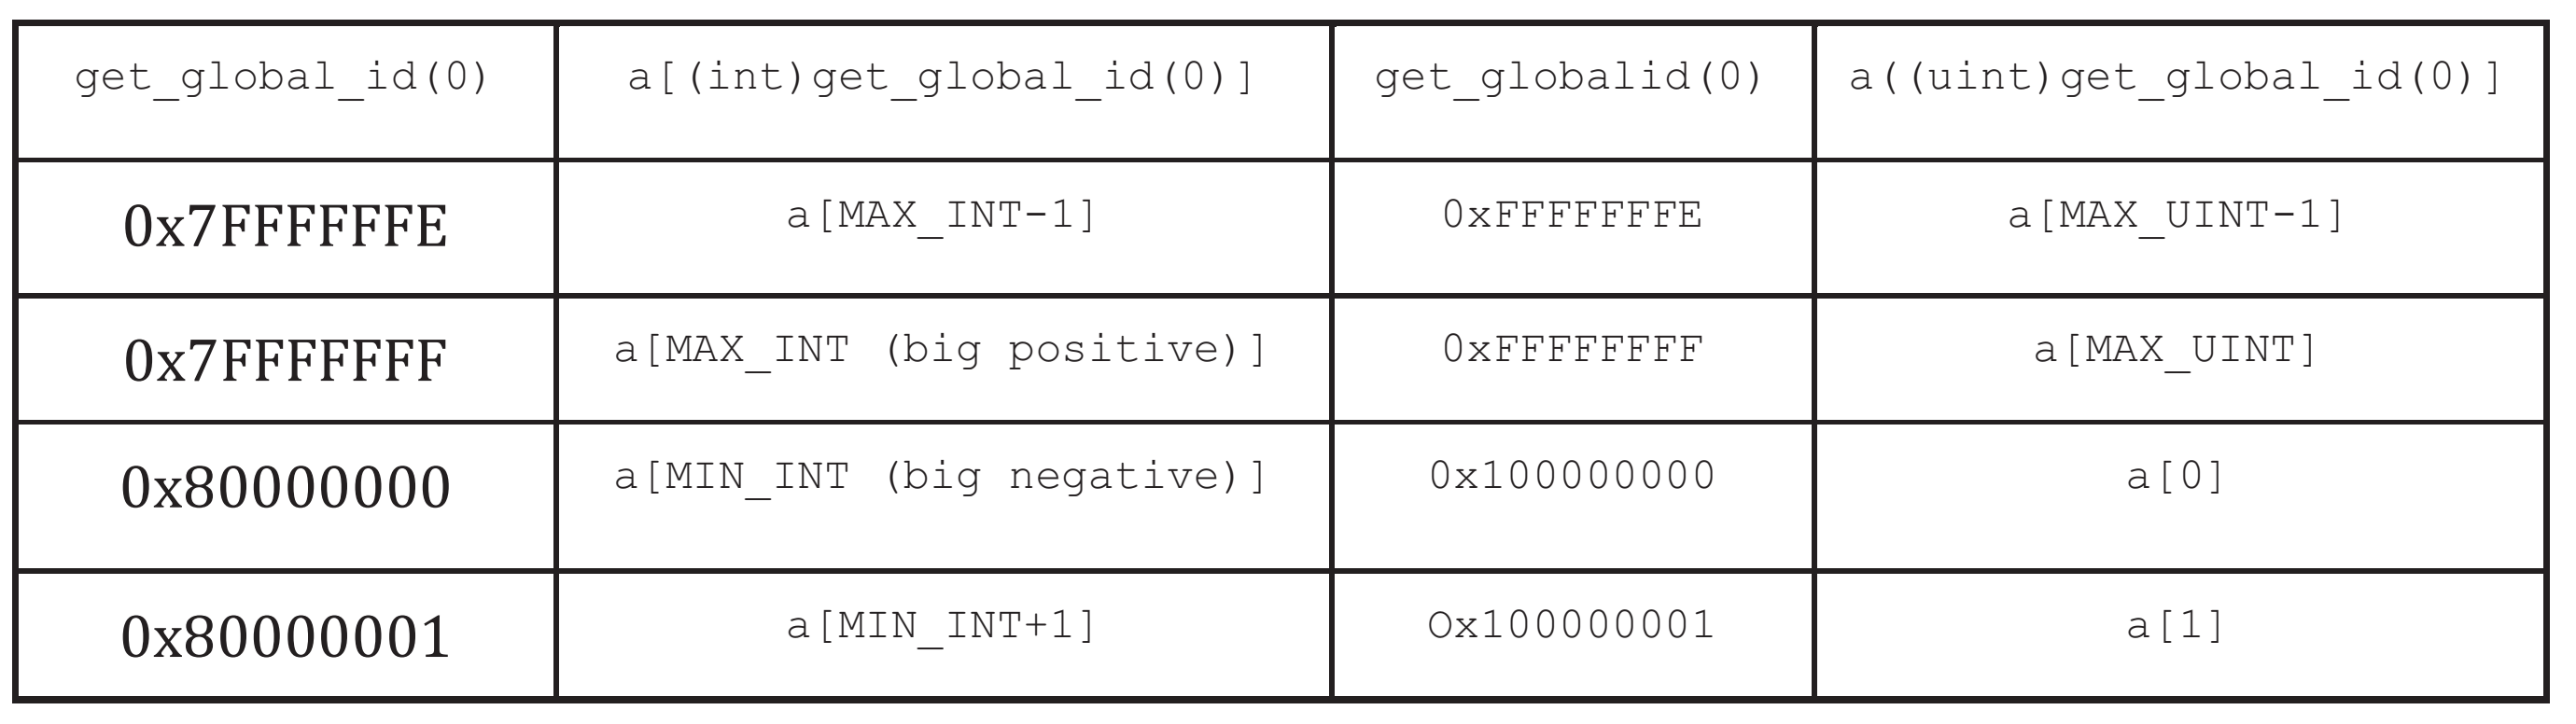
\includegraphics[width=1.0\textwidth]{content/chapter-16/images/12}
\end{center}

SIMD收集/分散指令比SIMD单元跨矢量加载/存储操作慢。为了最佳的SIMD效率,避免聚集/分散对于应用程序来说是至关重要的,无论使用哪种编程语言。\par

大多数SYCL get\_*\_id()函数有相同的问题,尽管许多情况下适用于MAX\_INT,因为返回值是有界的(例如,一个工作组中的最大id)。只要是合法的,DPC++编译器就会假定跨相邻工作项的单元跨内存地址,以避免聚集/分散。由于全局id和/或全局id的值可能溢出,编译器无法安全地生成单位跨距向量内存加载/存储操作,编译器将生成聚集/散点操作。\par

为用户提供最佳性能的理念下,DPC++编译器假定没有溢出,并且在实践中捕获真实状态,因此编译器可以生成最佳的SIMD代码以获得良好的性能。D\_\_SYCL\_DISABLE\_ID\_TO\_INT\_CONV\_\_是DPC++编译器用来告诉编译器会发生溢出的宏,使用id查询向量的访问可能不安全,这可能会对性能产生很大影响。这个宏应该在不安全的情况下使用,以假定没有溢出发生。\par

\hspace*{\fill} \par %插入空行
\textbf{使用single\_task执行SIMD}

单个任务执行模型中,向量类型和函数相关的优化依赖于编译器。编译器和运行时可以自由地支持显式SIMD执行或在single\_task内核中选择标量执行,结果取决于编译器实现。例如,DPC++ CPU编译器将为向量类型生成SIMD指令。vec加载、存储和swizzle函数将直接对向量变量执行操作,通知编译器数据元素正从内存中的相同(统一)位置开始访问连续数据,并能够请求优化的连续数据加载/存储。\par

\hspace*{\fill} \par %插入空行
图16-18 single\_task内核中使用向量类型和混合操作
\begin{lstlisting}[caption={}]
queue Q;
bool *resArray = malloc_shared<bool>(1, Q);
resArray[0] = true;

Q.single_task([=](){
	sycl::vec<int, 4> old_v = sycl::vec<int, 4>(000, 100, 200, 300);
	sycl::vec<int, 4> new_v = sycl::vec<int, 4>();
	
	new_vb.rgba() = old_v.abgr();
	int vals[] = (300, 200, 100, 000);
	
	if (new_v.r() != vals[0] || new_v.g() != vals[1] ||
	    new_v.b() != vals[2] || new_v.a() != vals[3]) {
      resArray[0] = false;    
    }
}).wait();
\end{lstlisting}

如图16-18所示,执行单个任务时,声明了一个包含三个数据元素的vector。使用old\_v.abgr()执行混合操作。如果CPU为混合操作提供SIMD硬件指令,那么可以通过在程序中使用混合操作获得一些性能收益。\par

\begin{tcolorbox}[colback=blue!5!white,colframe=blue!75!black, title=SIMD向量化指南]
CPU处理器用不同的SIMD宽度实现SIMD指令集。这是一个实现细节,并且对在CPU上执行内核的应用程序是透明的,因为编译器可以确定要用特定的SIMD大小处理的一组有效的数据元素,而不要求显式地使用SIMD指令。子工作组可以更直接地表示数据元素的分组,应受内核中SIMD执行的影响。\\

考虑到计算复杂度,选择最适合向量化的代码和数据布局最终可能会带来更高的性能收益。选择数据结构时,尽量选择数据布局、对齐方式和数据宽度,使最频繁执行的计算能够以对SIMD友好的方式访问内存,并具有最大的并行性。
\end{tcolorbox}








